% Created 2021-03-31 Wed 09:31
% Intended LaTeX compiler: pdflatex
\documentclass[12pt,paper=a4,oneside,hidelinks,headings=small,captions=heading,captions=nooneline]{scrartcl}
                \usepackage{microtype}
                \usepackage{tgpagella}
                \usepackage[scale=.9]{tgheros}
                \usepackage{tgcursor}
                \usepackage{paralist}
                \newcommand{\rc}{$^{14}C$}
\usepackage[utf8]{inputenc}
\usepackage[T1]{fontenc}
\usepackage{graphicx}
\usepackage{grffile}
\usepackage{longtable}
\usepackage{wrapfig}
\usepackage{rotating}
\usepackage[normalem]{ulem}
\usepackage{amsmath}
\usepackage{textcomp}
\usepackage{amssymb}
\usepackage{capt-of}
\usepackage{hyperref}
\usepackage[T1]{fontenc} %\hypersetup{colorlinks=true}
\usepackage{titlesec} \usepackage{lipsum}\usepackage{indentfirst}\setlength{\parindent}{3em}
\usepackage[tmargin=2.5cm, bmargin=2cm,inner=2.5cm,outer=2.5cm]{geometry}
\usepackage[sfdefault]{libertine} % sans = Linux Biolinum
\usepackage{fancyhdr}\pagestyle{fancyplain}\fancyhf{}
\renewcommand{\plainheadrulewidth}{0pt}\fancyhead[R]{\thepage}
\renewcommand{\headrulewidth}{0pt}
\renewcommand*\oldstylenums[1]{{\fontfamily{fxlj}\selectfont #1}}
\usepackage{lmodern}
\titleformat{\section}{\normalfont\centering\bfseries}{\thesection}{1em}{}
\titleformat{\subsection}{\normalfont\bfseries}{\thesubsection}{1em}{}
\titleformat{\subsubsection}{\normalfont\bfseries\itshape}{\thesubsubsection}{1em}{}
\titleformat{\paragraph}[runin]{\normalfont\bfseries}{\theparagraph.}{1em}{}[.]\titlespacing{\paragraph}{\parindent}{0pt}{4pt}
\titleformat{\subparagraph}[runin]{\normalfont\bfseries\itshape}{\thesubparagraph.}{1em}{}[. ]\titlespacing{\subparagraph}{\parindent}{0pt}{4pt}
\titleformat{\subsubparagraph}[runin]{\normalfont}{\thesubsubparagraph.}{1em}{}[. ]\titlespacing{\subsubparagraph}{\parindent}{0pt}{4pt}
\usepackage[hidelinks=true]{hyperref}
\usepackage[margin=1em,justification=centering]{caption}
\usepackage[ngerman, germanb]{babel}
\usepackage[utf8]{inputenc}
\usepackage[fixlanguage]{babelbib}\selectbiblanguage{austrian}
\usepackage{csquotes,xpatch}
\usepackage[natbib=true,style=apa,backend=biber,doi=true,url=true,eprint=false,hyperref=true,annotation=false]{biblatex}
\urlstyle{sf}
\DeclareLanguageMapping{austrian}{austrian-apa}
\DeclareSourcemap{\maps[datatype=bibtex]{\map{\step[fieldset=annotation,null]}}}
\addtolength\parskip{\medskipamount}
\usepackage{tabulary,booktabs,longtable}
\usepackage{caption}
\DeclareCaptionLabelSeparator{skipsep}{\vskip 1em} % APA 7 caption
\captionsetup[figure]{labelsep=skipsep}
\captionsetup[table]{labelsep=skipsep}
\addtokomafont{caption}{\itshape} % APA 7 italic figure/table captions
\setkomafont{captionlabel}{\normalfont\bfseries} % APA 7 bold figure/table caption labels
\renewcommand*{\captionformat}{\vskip 1.5em} % APA 7 caption
\setcaphanging
\setcapmargin*{0cm}
\setcapindent*{0pt}
\captionsetup{belowskip=1.5em,aboveskip=1.5em}% APA 7 distance between caption and figure/table
\BeforeBeginEnvironment{figure}{\vskip 1.5em}\AfterEndEnvironment{figure}{\vskip 1.5em}
\BeforeBeginEnvironment{table}{\vskip 1.5em}\AfterEndEnvironment{table}{\vskip 1.5em}
\AtBeginEnvironment{tabular}{\small}%
\author{Asım OĞUZ, Dominik PEGLER, Sophia PUM}
\date{\today}
\title{Meilenstein 1\\\medskip
\large HCI 2021S: Interior Designer}
\hypersetup{
 pdfauthor={Asım OĞUZ, Dominik PEGLER, Sophia PUM},
 pdftitle={Meilenstein 1},
 pdfkeywords={},
 pdfsubject={},
 pdfcreator={Emacs 27.1 (Org mode 9.4.4)}, 
 pdflang={Germanb}}
\begin{document}

\maketitle
\setcounter{tocdepth}{2}
\tableofcontents\newpage

\section{Literaturrecherche}
\label{sec:org7538986}
\emph{Autor: Dominik PEGLER}
\subsection{Automated interior design using a genetic algorithm (Kán \& Kaufmann, 2017)}
\label{sec:orga6b8437}

Kán und Kaufmann von der TU Wien stellen in dieser Arbeit aus dem
Bereich des Automated Interior Design ein Verfahren vor, das auf Basis
von vorgegebenen Informationen wie Raumgröße in der Lage ist,
virtuelle Räume automatisch und selbstständig mit Möbeln und
Einrichtungsgegenständen zu befüllen.

Dabei werden deren jeweilige Position und Ausrichtung im Raum so
gestaltet, dass sie ästhetischen, ergonomischen und funkionellen
Anforderungen optimal Rechnung tragen. Diese Anforderungen nennen sich
Interior Design Guidelines.

Sie wurden für dieses Verfahren in mathematische Ausdrücke übersetzt
und in eine Kostenfunktion integriert. Mittels eines Genetischen
Algorithmus (GA) wird diese Kostenfunktion auf ein Minimum
optimiert. Zusätzlich eweitert dieses Verfahren auch die Optimierung
auf den transdimensionalen Raum: dadurch wird die automatische Auswahl
von Gegenständen möglich. Ebenfalls optimiert wird die Zuordnung von
Materialien zu den Möbeln und Einrichtungsgegenständen, um ein
einheitliches Design und eine harmonische Farbgestaltung zu
erreichen.

In einer Wahrnehmungsstudie wurde festgestellt, dass dieses Verfahren
tatsächlich in der Lage ist, lebenswerte und sinnhafte
Innenarchitekturen zu generieren. Im Vergleich zu von professionellen
Designern generierten Layouts schnitten die automatisch generierten
Layouts gut ab, wobei Küchen deutlich besser und Schlafzimmer deutlich
schlechter bewertet wurden als jene der professionellen
Innenarchitekten.

\subsection{Augmented reality uses in interior design (Sandu, M., \& Scarlat, I. S., 2018)}
\label{sec:org1e811a6}

Weil Möbel zunehmend über Online-Shops gekauft werden und sich viele
Kunden in der Folge nicht vorstellen können, wie neue Möbelstücke in
ihrem Zuhause aussehen würden, lösen viele Unternehmen dies mit dem
Einsatz von Augmented Reality (AR) in ihren Applikationen.

AR-Anwendungen sind in der Lage, die virtuellen Möbel auf dem
Anwendungsbildschirm in eine physische Umgebung einzubetten, virtuelle
Markierungen im Raum zu machen und über diese Größe und
Größenverhältnisse im Koordinatensystem des Raums zu ermitteln. Der
Benutzer kann also virtuelle Möbel auf dem Bildschirm auswählen und an
einer beliebigen Stelle im Raum platzieren. Wesentlicher Bestandteil
bei AR-Anwendungen ist dabei die Kamera des Smartphones.

In dieser Arbeit werden verschiedene AR-Anwendungen für Interior
Design analysiert, dabei Vor- und Nachteile erhoben und in Folge eine
AR-Anwendung vorgeschlagen, die die meisten aktuellen Probleme der
Innenraumgestaltung löst.

Als Software-Frameworks für Augmented Reality wird ArToolKit
vorgestellt, ein vielfach verwendetess und minimales
Open-Source-Framework. Das ARToolKit-Tracking funktioniert wie folgt:

\begin{enumerate}
\item Kamera nimmt Videos der realen Welt auf und sendet ans Programm
\item Programm durchsucht alle quadratischen Formen in den Videos
\item Wird ein Quadrat gefunden, errechnet die Software die Position der
Kamera relativ zum schwarzen Quadrat.
\item Sobald die Position der Kamera bekannt ist, wird das
Modell aus dieser Perspektive gerendert.
\item Modell wird auf dem Video der realen Welt gezeichnet (auf einer
quadratischen Markierung).
\item Das fertige Bild wird am Display angezeigt, auf dem virtuelle
Gegenstände über die reale Welt gelagert sind.
\end{enumerate}

Als App, die auf AR-Technologien aufbaut, wird IKEA place application
genannt. Sie soll helfen, den Entscheidungsprozess beim Kauf von
Einrichtungsgegenständen zu erleichtern. Bei ihr liegen die
Fehlerbereich bei wenigen Zentimetern. Die App ist auch in der Lage,
physische Objekte im Raum zu erkennen und etwas Ähnliches aus dem
Online-Shop vorzuschlagen. Als Nachteil der IKEA-place-app wird
genannt, dass Objekte manchmal völlig inkorrekt oder in inkorrekter
Größe platziert. Ein weiterer Nachteil ist, dass nur Gegenstände aus
dem IKEA-eigenen Store ausgewählt werden können.

Eine weitere Applikation ist die Houzz-App. Im Gegensatz zur IKEA-App
 kann diese App besser flache Oberflächen erkennen, was die genannten
 groben Fehler verringern kann. Obwohl auch diese App nicht ohne
 Nachteile auskommt (Freezing, uneinheitliches
 Cross-Device-Verhalten), ist sie einer von den Autoren gestarteten
 Umfrage zufolge beliebter als die App von IKEA. Das wird vor allem
 auf das Design zurückgeführt.

Als eine den Autoren nach sehr gute Lösung wird auch noch die App
Homerstyler Interior Design genannt. Diese erlaubt auch
Größenänderungen der Objekte in Echtzeit, vordefinierte leere Räume
zu wählen und diese nach Belieben zu gestalten. Einziger Nachteil
dieser App ist der Umstand, dass kein kompletter Raum-Scan möglich
ist und nach der Umfrage ist sie wenig populär und liegt hinter
jener von IKEA.

Der Lösungsvorschlag der Autoren wäre eine App, die die Möglichkeit
bietet, nach dem Scan der Umgebung bestimmte Objekte oder alle Objekte
entfernen zu können. Damit lässt sich ein Raum leichter oder von Grund
auf neu gestalten. Es wäre auch eine Neuheit, da diese Funktion zum
Zeitpunkt des Artikels in keiner Smartphone-Anwendung verfügbar
war. Die Autoren schildern am Ende auch noch kurz, wie ein Algorithmus dafür
aussehen könnte.

\subsection{Inter AR: Interior decor app using augmented reality technology (Moares, R., Jadhav, V., Bagul, R., Jacbo, R., Rajguru, S., \& K, R., 2020)}
\label{sec:org01baab4}

In diesem Artikel beschreiben die Autoren die Vorgänge, die in
AR-basierten Interior-Design-Applikationen stattfinden. Ausgangspunkt
sind hier zwei Algorithmen, die die reale Umgebung erfassen: der
sogenannte Harris-und-Stephens-Ecken-Detektor-Algorithmus und der
SLAM-Algorithmus (surface localization and mapping) zur Erfassung der
Oberflächen.

Die Autoren nennen weiters fünf häufig verwendete Methoden von AR:

\begin{enumerate}
\item Markerbasierte AR (marker-based AR)

Verwendet visuelle Marker wie QR/2D-Codes oder NFT-Marker
(tatsächliche Gegenstände). Nach der Markererkennung und der
Kalkulation der Position und Ausrichtung wird der virtuelle
Gegenstand platziert.

\item Ortsbasierte AR (location-based AR)

Diese Form der AR ist weit verbreitet und verwendet anstelle von
Markern die im Gerät verbauten Sensoren zur Bestimmung der
Position.

\item Projektionsbasierte AR (projection-based AR)   

In diesem Verfahren wir Licht vom Gerät auf die Umgebung
geworfen. Die Ergebnisse lassen Rückschlüsse über Position,
Ausrichtung und Tiefe von Objekten zu.

\item Outlining AR

Diese Methode funktioniert mittels spezieller Kameras, die es
ermöglichen Aufnahmen der Umgebung bei schlechten
Lichtverhältnissen zu machen. Diese Methode hat Ähnlichkeit mit der
projektionsbasierten AR und kommt in Parkassistenten von Autos zur
Anwendung.

\item Überlagerungs-AR (superimposition-base AR)

Teilweise oder sogar vollständige Ersetzung der realen Umgebung
eines Objekts durch eine virtuelle Umgebung desselben Objekts.
\end{enumerate}

Im Rahmen dieses Artikels wurde eine AR-Applikation mittels
markerloser AR erstellt. Für die 3D-Modelle wurde das Google Cardboard
SDK verwendet.

Dabei wurden folgende Einschränkungen genannt: (1) Nicht alle
Android-Geräte unterstützen AR-Technologien vollständig. Es gibt zwar
Workarounds, doch sind diese nicht immer präzise. (2) Möbelobjekte
werden aus dem Backend importiert und lokal
gespeichert. Aufgrunddessen gibt es keine Photogrammetrie, mit der die
Anwendung das Bild in ein 3D-Objekt konvertieren kann. (3) Die
Anwendung erlaubt aufgrund der begrentenz Funktionen der Google
Entwicklertools keine Platzierung von zwei oder mehr Objektinstanzen
auf einer einzelnen Oberfläche.

Nichtsdestotrotz zeigte das Projekt, dass der Benutzer die virtuellen
Möbel nach den eigenen Vorstellungen anpassen und in der realen Welt
arrangieren kann. Über die Smartphone-Kamera kann der Benutzer die
Oberflächen erkennen, die Möbel über die App auswählen und nach Wunsch
auf dem Bildschirm platzieren. Eine Verknüpfung mit AI könnte für
verschiedene Zwecke in Zukunft eine Rolle spielen.

Die Arbeit soll helfen, Menschen die Möglichkeit zu geben, selbst
Designer zu sein und ihr Zuhause nach eigenen Vorstellungen zu
gestalten. Ein solches System hat den Autoren nach viele Vorteile,
weil dadurch auch bereits bekannte Limitationen von Möbelhäusern wie
z.B. begrenze Auswahl an lagernden Möbelstücken an Gewicht
verlieren.

\subsection{Quellen}
\label{sec:org1b0bd12}
\begin{itemize}
\item Kán, P. \& Kaufmann, H. (2017). Automated interior design using a
genetic algorithm. Proceedings of the 23rd ACM Symposium on Virtual
Reality Software and Technology,
1– 10. \url{https://doi.org/10.1145/3139131.3139135}
\item Moares, R., Jadhav, V., Bagul, R., Jacbo, R., Rajguru, S., \& K, R.,
Inter AR: Interior decor app using augmented reality technology
(2020). Social Science Research
Network. \url{https://papers.ssrn.com/abstract=3513248}
\item Sandu, M., \& Scarlat, I. S. (2018). Augmented reality uses in interior
design. Informatica Economica, 22(3/2018), 5-13. 
\url{http://dx.doi.org/10.12948/issn14531305/22.3.2018.01}
\end{itemize}
\section{Konkurrenzprodukte}
\label{sec:orgeb112b2}
\emph{Autorin: Sophia PUM}

Die wahrscheinlich bekannteste Interior-Design-App auf dem Markt ist
\textbf{Houzz} (Abb. \ref{fig:m1_ko_01}). Mit Millionen von qualitativen Bildern von Badezimmern,
Wohnzimmern, Küchen, Möbeln und wo weiter bietet sie den Nutzenden
viel Inspiration und die Möglichkeit sich einen Eindruck von
verschiedenen Einrichtungen und Farbkombinationen zu
schaffen. Praktisch ist die Funktion, dass man sich eigene persönliche
Entwürfe speichern kann. Außerdem kann man sich auch mit einer
User-Community austauschen und gegenseitig inspirieren.

Der größte Vorteil der App ist die große Menge an Bildern von
Gestaltungsmöglichkeiten in verschiedenen Stilen, die sie
beinhaltet. Nutzer verwenden Sie vor allem um sich Inspiration zu
holen.

Ein Nachteil ist, dass sich die App Großteiles auf die Einrichtung von
Häuser und Hausbau spezialisiert. Obwohl sie angibt für alle Wohnungen
geeignet zu sein, findet man auf den Fotos auch hauptsächlich große,
helle Räume. Das ist vor allem für junge Leute, die oft in kleinen
Wohnungen oder WG-Zimmern wohnen unpraktisch.

Generell ist die App nicht wirklich auf junge Leute ausgerichtet und
könnte sich in der Hinsicht verbessern. Denn diese nutzen oft schon
bekannte Apps wie Instagram oder Pinterest zur Inspiration. Für sie
hat es dann wenig Sinn eine zusätzliche App herunterzuladen, die nicht
einmal ihre Wünsche abdeckt. Das ist meiner Meinung nach definitiv ein
Nachteil, denn gerade Anfang 20 ziehen viele Menschen um und wären
potentielle Nutzerinnen und Nutzer einer Einrichtungs-App.

\begin{figure}[htbp]
\centering
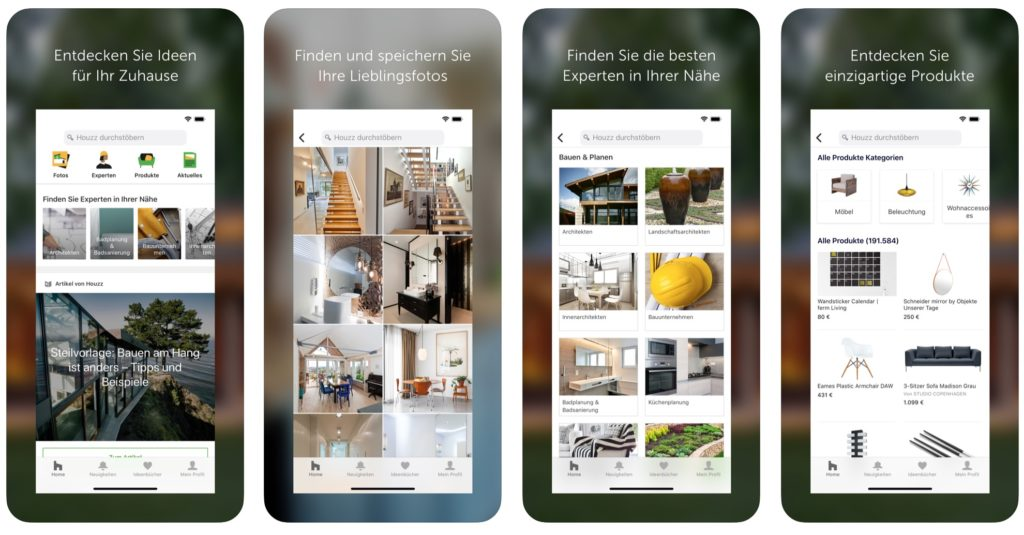
\includegraphics[height=200px]{./img/m1_konkurrenzanalyse_01.jpg}
\caption{\label{fig:m1_ko_01}Houzz App}
\end{figure}

\textbf{Ikea Place} ist die Einrichtungs-App vom Möbelhaus Ikea (Abb. \ref{fig:m1_ko_02}). Mithilfe einer
Augumented-Reality-Technologie kann man sehen wie die Ikea-Produkte in
den eigenen Räumlichkeiten aussehen würden. Die Gegenstände werden
dreidimensional und maßstabsgetreu nachgestellt. Zusätzlich gibt die
App auch Tipps zur Einrichtung. Das Ziel der App ist es, dass sich
jeder von zuhause aus einen besseren Eindruck von den Möbeln machen
kann.

Der größte Vorteil der App, ist meiner Meinung nach, dass alle
Funktionen und Produkte von Ikea ist. Man kann sich die Möbel von
zuhause aus ansehen und hat durch die moderne Technologie einen guten
Einblick drauf, wie sie in die Wohnung passen würden. Im
Ikea-Onlineshop kann man die Produkte im Anschluss sofort bestellen
und sich liefern lassen. So erfolgt das Einrichten rasch und
unkompliziert.

Allerdings hat Ikea hauptsächlich Möbel im modernen-skandinavischen
Stil und Nutzende haben nicht die Möglichkeit verschiedene
Gestaltungsarten auszuprobieren. Außerdem kann man nur eine
beschränkte Anzahl der Ikea-Produkte in der Ikea Place App verwenden.

\begin{figure}[htbp]
\centering
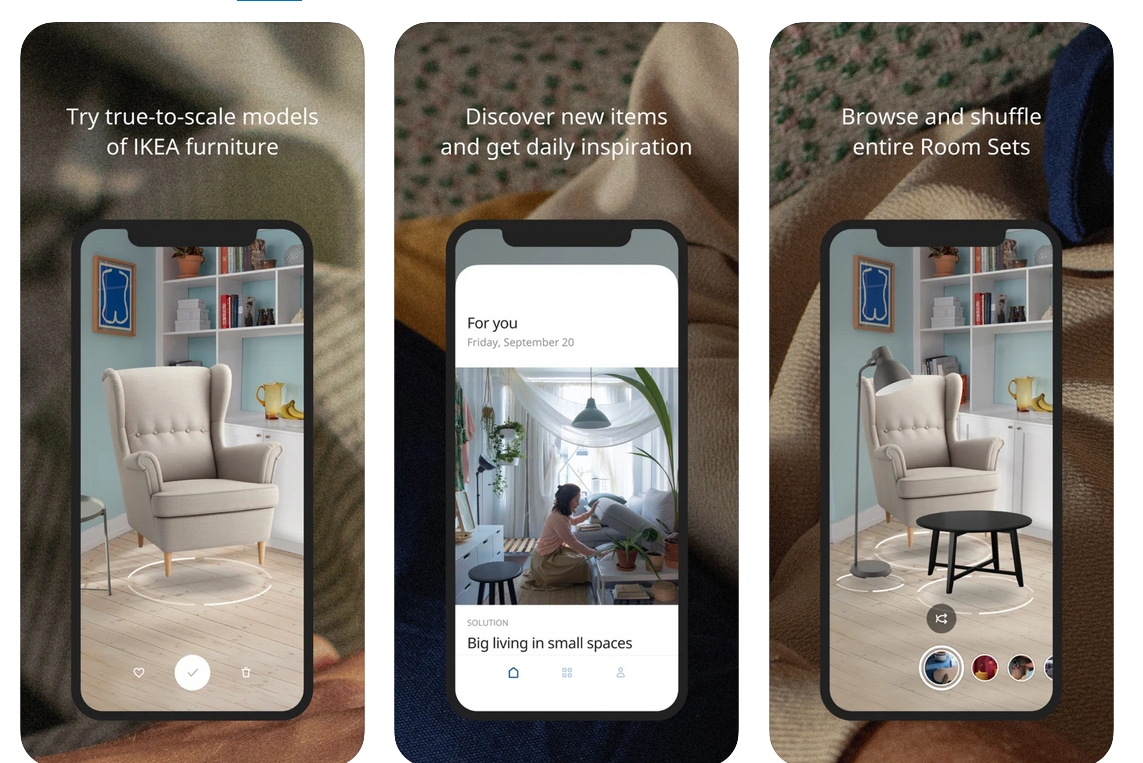
\includegraphics[height=200px]{./img/m1_konkurrenzanalyse_02.jpg}
\caption{\label{fig:m1_ko_02}Ikea Place App}
\end{figure}

Auch bei \textbf{Homestyler Interior Design \& Deko-Ideen} (Abb. \ref{fig:m1_ko_03}) kann man Fotos von
seinen Räumlichkeiten in die App laden und mit einer großen Menge an
Farben, Materialien und Möbel bearbeiten und umgestalten. Sie bietet
eine gute Einsicht darauf, wie sich gewisse Änderungen im Raum machen
würden. Auch hier gibt es eine User-Community zum Austausch von Ideen
und Entwürfen.

Die App bietet viele Gestaltungsmöglichkeiten und ist einfach zu
handhaben. Sie enthält 3D-Modellen von Möbeln verschiedener Marken,
und bietet so die Möglichkeit viele verschiedene Stile auszuprobieren

Ein Feature an dem es der App aber fehlt, ist die Möglichkeit einen
leeren Raum zu erstellen um seine Ideen komplett neu zu entfalten.

\begin{figure}[htbp]
\centering
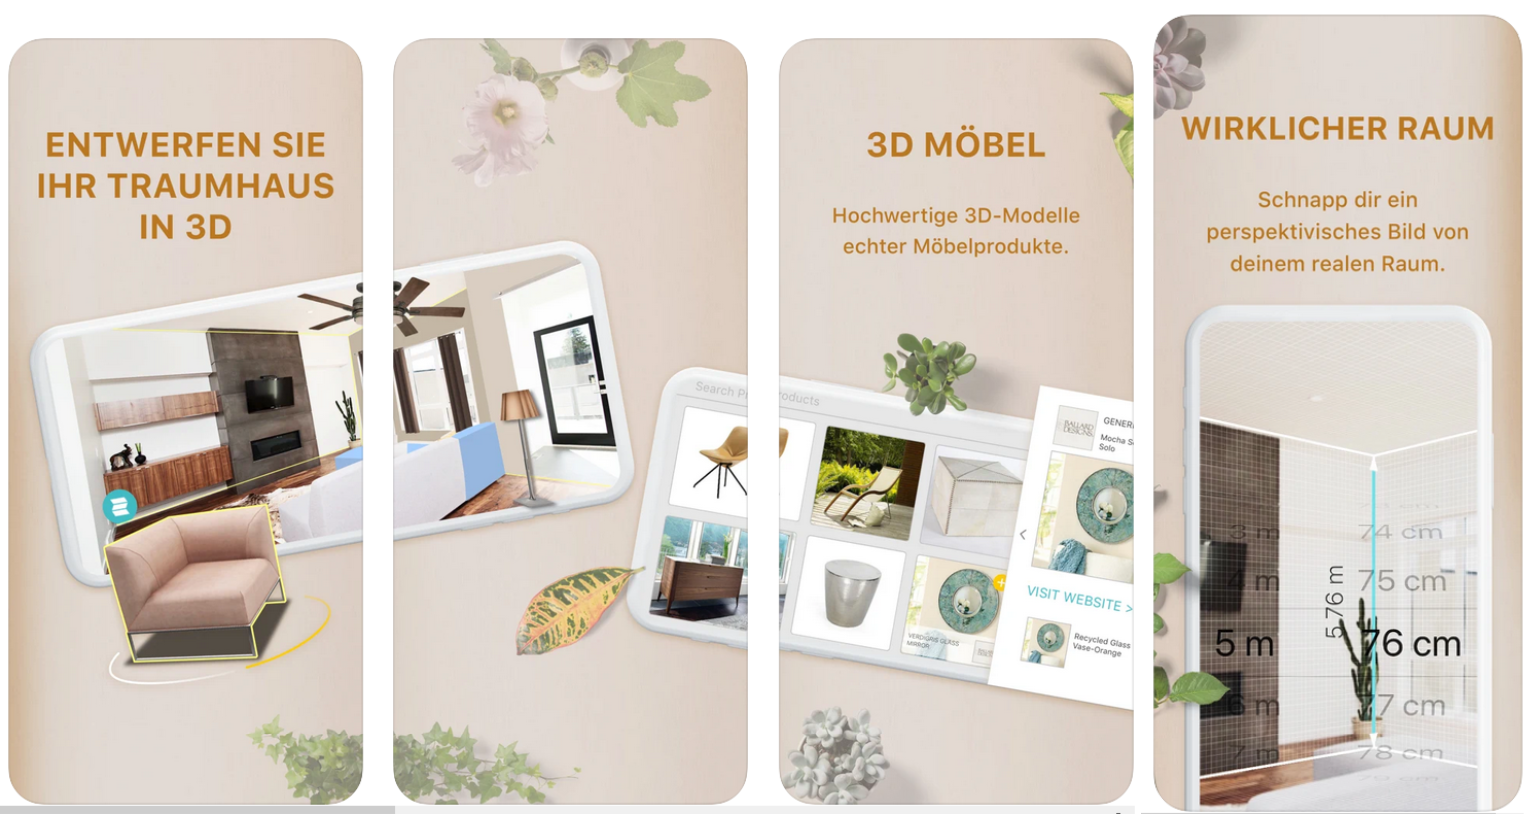
\includegraphics[height=200px]{./img/m1_konkurrenzanalyse_03.png}
\caption{\label{fig:m1_ko_03}Homestyler App}
\end{figure}

\section{Nutzer- \& Kontextanalyse}
\label{sec:orgaed35f1}

\subsection{Nutzeranalyse}
\label{sec:org32a7d97}
\emph{Autor: Dominik PEGLER}
\subsubsection{Aufgaben der Nutzer}
\label{sec:org6b70dd7}
\begin{itemize}
\item Schnelles und unkompliziertes Skizzieren von Innenarchitekturen
\item Schnelle und unkomplizierte Visualisierung der gestalteten Innenarchitekturen
\item Die eigenen Vorstellungen anderen Personen einfach und anschaulich
zu kommunizieren
\end{itemize}

\subsubsection{Ziele der Nutzer}
\label{sec:org0215048}
\begin{itemize}
\item Zeit- und Kostenersparnis, weil keine Beratung durch
Innenarchitekt*in nötig ist und die App an Ort und Stelle hilfreich
ist
\item Konkretere Vorstellungen zu entwickeln
\item Bessere und nachhaltigere Entscheidungen zu treffen
\end{itemize}

\subsubsection{Potenzielle Probleme mit dem System}
\label{sec:org84205a6}
\begin{itemize}
\item Die User fühlen sich von der App nicht angesprochen.
\item Die Funktionalitäten oder Auswahlmöglichkeiten sind zu
eingeschränkt, z.B. gibt es nur eine bestimmte Art von Möbeln oder
Objekten, die über die App darstellbar sind, oder es gibt technische
Limitationen mehre virtuelle Objekte gleichzeitig darzustellen.
\item Die User sehen den Nutzen nicht (wegen Art des Aufbaus der App nicht
klar ersichtlich)
\item App bringt keinen Zusatznutzen zu bereits vorhandenen Tools
\item User können Aufbau und Logik des Programms nicht nachvollziehen
\item Zu lange Ladezeiten (bei mobilen Apps noch wichtiger als bei Webapps!)
\item Freezing oder Absturz der App
\item Smartphone genügt den Anforderungen nicht
\end{itemize}

\subsubsection{Userpfade:}
\label{sec:org8c045cc}
\begin{itemize}
\item \textbf{Wie können User die App downloaden?}

Über den jeweiligen Appstore oder über einen Link, der von einer
dritten Person zugesendet wird.

\item \textbf{Welche Hilfestellungen werden mit der App mitgeliefert?}

Eigener Menüpunkt, der zu einer mobilen Hilfeseite mit Problem-Kategorien
und einer Suchfunktion führt.

\item \textbf{Wie sieht die Erstbenutzung aus?}

Es sind keinerlei Registrierungen notwendig. Die Nutzer gelangen
sofort in ein Menü, in dem sie die gewünschte Aktion auswählen
können. Es sollte möglich sein, bereits 5 Bildschirmberührungen ein
Ergebnis zu bekommen. Zum Beispiel mittels Defaulteinstellungen.

\item \textbf{Was sind die Anreize, die App wiederzuverwenden?}

Gute Ersterfahrungen sind der wichtigste Grund, die App
wiederzuverwenden. Die Ersterfahrung muss bereits den Nutzen der App
demonstrieren und zu einem Erfolgserlebnis führen.
\end{itemize}

\subsubsection{Nutzergruppen}
\label{sec:org975a417}

Die User teilen sich auf viele große Gruppen auf, da es sich beim
Thema Wohnen um etwas handelt, das jeden von uns betrifft und die
meisten Menschen in der Lage sind, ihre Wohnsituation selbst zu
gestalten. Aus diesem Grund sind Kinder und Jugendliche unter 15
Jahren sind mit großer Wahrscheinlich weniger stark vertreten, ebenso
sehr alte Personen und Personen mit starken neurobiologischen
Beeinträchtigungen.

\paragraph{Kategorienbildung nach Alter und Fachwissen}
\label{sec:org94989de}

Der Vorteil dieser Kategorisierung (siehe Tabelle \ref{tbl:usergroups})
liegt darin, dass Alter und Expertise wahrscheinlich stark mit der Art
der Nutzung von Smartphones (Phänomen aus den letzten 15 Jahren) und
speziellen Tools zusammenhängt. Alter ist einfacher zu erfassen als
Smartphone literacy.

\begin{table}[htbp]
\caption{\label{tbl:usergroups}Die Nutzergruppen nach Alter und Fachwissen im Überblick}
\centering
\begin{tabular}{ll}
\toprule
ID & Nutzergruppe\\
\midrule
J & Jüngere Menschen (15--35 Jahre) ohne professionellen Background im Bereich Innenarchitektur\\
M & Menschen im mittleren Alter (36--60 Jahre) ohne professionellen Background\\
A & Ältere Menschen (60--80 Jahre) ohne professionellen Background\\
JM+ & Menschen im jungen oder mittleren Alter mit professionellem Background\\
A+ & Ältere Menschen mit professionellem Background\\
\bottomrule
\end{tabular}
\end{table}

\paragraph{Mögliche andere Kategorienbildung}
\label{sec:org48ea9c1}
\begin{itemize}
\item Bildung
\item Einkommen
\item Smartphone/Computer literacy
\end{itemize}

\subsection{Kontextanalyse}
\label{sec:orgb6062df}

\begin{itemize}
\item Benutzer hat keine Vorstellung von möglichen innenarchitektonischen
Designs
\item Benutzer hat keine professionellen Kenntnisse und keine Tools zur
Veranschaulichung zur Hand
\item Benutzer hat auch sonst keine ergänzenden Hilfsmittel wie
Zeichenstifte und Papier zur Hand
\item Benutzer besitzt ein Smartphone auf dem aktuellen Stand der Technik
\item Bedarf zur Verwendung der App
\begin{itemize}
\item entsteht außerhalb von professionellen Settings
\item kann fast an jedem Ort und Situation entstehen
\end{itemize}
\end{itemize}

\section{Personas}
\label{sec:org8566c8f}

\subsection{Primäre Persona \#1}
\label{sec:org85540ab}

\emph{Autor: Asım OĞUZ}

\begin{figure}[htbp]
\centering

\includegraphics[width=110px]{./img/m1_persona_1_idealist.png}
\caption{\label{fig:persona1}"`Tobias Ebner"'}
\end{figure}

\begin{itemize}
\item Name: Tobias Ebner
\item Typ: Idealist
\item Credo: \emph{Mit minimalem Aufwand maximalen Erfolg erreichen}
\item Background:

Tobias Ebner, der 25 Jahre alt ist, hat vor kurzem seine
Ausbildung abgeschlossen und arbeitet nun als Vollzeit Grafik
Designer. Da er jetzt ein höheres Budget zur Verfügung hat will er
aus der WG ausziehen und zum ersten mal in seinem Leben alleine
leben. Wie sein Job es auch vermuten lässt mag Tobias Ebner gut
durchdachte Designs, daher ist es ihm auch wichtig vor dem Umzug
alles so gut wie möglich durch zu planen.  Tobias Ebner erleichtert
sich immer die Arbeit in dem er sich nützliche Tools findet.

\item Abneigung: Zeitverlust
\item Männlich, 25 Jahre
\item Nationalität: Österreich
\item Familienstand: Single
\item Beruf: Grafik-Designer
\item Berufserfahrung: 1 Jahr
\item Einkommen: EUR 30.000 / Jahr
\item Nutzung mobiler Geräte: 8h / Tag
\item Verwendete Technologien: Android Smartphone, iPad, Windows-Laptop,
Windows-Desktop-PC
\end{itemize}

\subsection{Primäre Persona \#2}
\label{sec:orgbb46d01}

\emph{Autorin: Sophia PUM}

\begin{figure}[htbp]
\centering
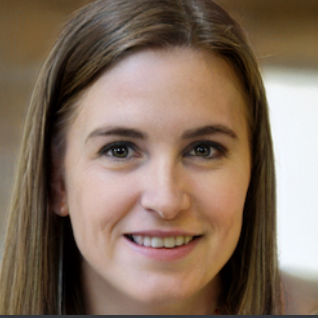
\includegraphics[width=110px]{./img/m1_persona_2_rational.png}
\caption{\label{fig:persona2}"`Carina Winkler"'}
\end{figure}

\begin{itemize}
\item Name: Carina Winkler
\item Typ: Rational
\item Background:

Carina Winkler ist 32 Jahre alt, verheiratet und arbeitet als Ärztin
in einer Arztpraxis in Wien. Nun möchte sie ihren Traum
verwirklichen und gemeinsam mit ihrem Mann eine eigene Arztpraxis
eröffnen. Außerdem wollten sie und ihr Ehemann schon lange aus ihrer
kleinen Wohnung in der Wiener Innenstadt ausziehen und in ein Haus
außerhalb der Stadt ziehen. Ihr Plan ist es, ein Haus mit Arztpraxis
und privatem Wohnbereich einzurichten. Da beide beruflich viel zu
tun haben und sich zusätzlich nicht zu viel mit dem Umzug stressen
wollen, freuen sie sich über jede Art von Unterstützung. Ihr Wunsch
ist ein Umzug der unkompliziert sowie stressfrei verläuft, aber
trotzdem ihre Wohnträume erfüllt. Sie ist bereit, sich Zeit zu
nehmen und den Umzug inklusive der Einrichtung gut zu planen, damit
es zu keinen unüberlegten Entscheidungen kommt und sie mit dem
Endergebnis langfristig zufrieden ist. Carina ist offen dafür Neues
auszurobieren, solange es zu einer effizienteren Problemlösung
beiträgt und keine zusätzlichen Schwierigkeiten bedeutet.

\item Ziele:
\begin{itemize}
\item Ein unkomplizierter, effizienter Umzug
\item Eine Einrichtung, die langfristig gefällt
\item Neues ausprobieren, ohne viel zu riskieren
\end{itemize}
\item Motivation:
\begin{itemize}
\item Übersichtlich organisierte Pläne
\item Praktische Herangehensweise
\end{itemize}
\item Abneigung:
\begin{itemize}
\item Strukturlosigkeit
\item Unüberlegte und hektische Entscheidungen
\end{itemize}
\item Weiblich, 32 Jahre
\item Nationalität: Österreich
\item Familienstand: Verheiratet
\item Beruf: Ärztin
\item Berufserfahrung: nicht bekannt
\item Einkommen: EUR 60.000 / Jahr
\item Nutzung mobiler Geräte: nicht bekannt
\item Verwendete Technologien: iPhone, iPad, Windows-Laptop,
Windows-Desktop-PC
\end{itemize}

\subsection{Sekundäre Persona:}
\label{sec:orgc63318a}

\emph{Autorin: Sophia PUM}

\begin{figure}[htbp]
\centering

\includegraphics[width=110px]{./img/m1_persona_3_rational.png}
\caption{\label{fig:persona3}"`Felix Schuster"'}
\end{figure}

\begin{itemize}
\item Name: Felix Schuster
\item Typ: Rational
\item Background:

Felix Schuster ist 20 Jahre alt und zum Studieren nach Wien
gezogen. Er hat ein günstiges WG-Zimmer im Internet gefunden und
zieht das erste Mal von zuhause weg. Felix ist extravertiert und
viel unterwegs, entweder zum Lernen auf der Bibliothek oder er
unternimmt etwas mit Freunden. Sein Wohnraum dient hauptsächlich zum
Schlafen und er ist selten zuhause. Er möchte sich sein Zimmer schön
einrichten und sich darin wohlfühlen, allerdings hat es für ihn
keinen hohen Stellenwert und dient auch nicht zur
Selbstverwirklichung. Er möchte flexibel bleiben und wird
voraussichtlich nur für ein paar Jahre dort wohnen, somit will er
nicht zu viel Zeit oder Geld mit der Gestaltung seines Zimmers
verschwenden. Grundsätzlich ist er aber ein offener und moderner Typ
und probiert auch gerne Neues aus, allerdings mag er es gerne
unkompliziert und bequem.

\item Ziele:
\begin{itemize}
\item Ein unaufwändiger Umzug
\item Eine minimalistische Einrichtung, die das Nötigste abdeckt
\item Neues ausprobieren, ohne zu viel zu riskieren
\end{itemize}
\item Motivation:
\begin{itemize}
\item Interessiert an modernen Trends
\item Bequeme Herangehensart
\item Spontane Entscheidungen
\end{itemize}
\item Abneigung:
\begin{itemize}
\item Strenge Pläne und Vorschriften
\item Eingeschränkte Möglichkeiten
\end{itemize}
\item Männlich, 20 Jahre
\item Nationalität: Österreich
\item Familienstand: Single
\item Beruf: Student
\item Berufserfahrung: nicht bekannt
\item Einkommen: -
\item Nutzung mobiler Geräte: nicht bekannt
\item Verwendete Technologien: Android Smartphone, Windows-Laptop
\end{itemize}

\subsection{Negative Persona}
\label{sec:orge806d6e}

\emph{Autor: Asım OĞUZ}

\begin{figure}[htbp]
\centering
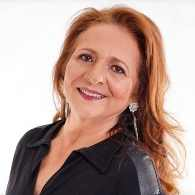
\includegraphics[width=110px]{./img/m1_persona_4_guardian.jpg}
\caption{\label{fig:persona4}"`Sabine Gruber"'}
\end{figure}

\begin{itemize}
\item Name: Sabine Gruber
\item Typ: Guardian
\item Credo: \emph{Der beste Weg ist der, den man kennt}
\item Background:

Sabine Gruber ist eine 64-jährige Verkäuferin, die schon seit mehr
als 20 Jahren im selben Geschäft in derselben Stelle
arbeitet. Sabine Gruber ist verheiratet und lebt mit ihrem Ehemann
zusammen in Wien. Das Umsteigen auf Neues fällt ihr sehr schwer und
daher mag sie es auch nicht, Neues auszuprobieren. Wenn sie mal
etwas findet, das ihr gefällt, hält sie sehr lange daran fest, seien
es Gegenstände als auch Designs.

\item Abneigung: Etwas Neue ausprobieren
\item Weiblich, 64 Jahre
\item Nationalität: Österreich
\item Familienstand: Verheiratet
\item Beruf: Verkäuferin
\item Berufserfahrung: 37 Jahre
\item Einkommen: EUR 22.000 / Jahr
\item Nutzung mobiler Geräte: 2h / Tag
\item Verwendete Technologien: iPhone
\end{itemize}
\section{Aufgabenanalyse}
\label{sec:org0c54022}
Die Aufgabenanalyse (siehe Tabelle \ref{tbl:task_analysis}) veranschaulicht in Form von Use-Cases für die
primären Personas die Wichtigkeit der einzelnen Aufgaben, die die User
haben, um zum Resultat zu kommen.

\emph{Autor: Asım OĞUZ}

\begin{table}[htbp]
\caption{\label{tbl:task_analysis}Bisherige Aufgabenverteilung}
\centering
\begin{tabular}{lll}
\toprule
Task\User & Carina Winkler & Tobias Ebner\\
\midrule
App downloaden & + & +\\
Raum fotografieren & + & +\\
Möbel scannen & \textasciitilde{} & \textasciitilde{}\\
Vorhandene Möbel auswählen & + & +\\
Raum gestalten & \textasciitilde{} & \textasciitilde{}\\
Design abspeichern & + & +\\
\bottomrule
\end{tabular}
\end{table}

\section{Projektmanagement}
\label{sec:org0bba3bf}

\emph{Autor: Dominik PEGLER}

Für das Projekt-Management haben wir auf github eine einfache
HTML-Seite (\url{https://dominikpegler.github.io/interior-designer}) erstellt, auf der man sich über den aktuellen Stand des
Projekts informieren kann und die nächsten wichtigen Termine wie
Meilensteine und Präsentationen bekommt. Über das gesame Projekt wird
hier Buch geführt, außerdem entsteht im selben github-Repository (\url{https://github.com/dominikpegler/interior-designer}) der
Source-Code der App. All diese Dinge sind öffentlich zugänglich.

\subsection{Team}
\label{sec:orgcd141d3}

Das Team besteht aus \textbf{Asım Oğuz} und \textbf{Sophia Pum}, beide studieren
im 4. Semester des Bachelorstudiums Informatik, sowie aus \textbf{Dominik
Pegler}, Student im letzten Bachelor-Semester Psychologie. Für die
Aufteilung der Tätigkeiten sind wir so vorgegangen, dass wir
untereinander vorab abgeklärt haben, über welches Wissen und welche
Fähigkeiten jedes Mitglied der Gruppe verfügt und was es im Laufe der
Lehrveranstaltung verbessern möchte. Sophia Pum ist kreative
Ideengeberin im Projekt und auch wesentlich in die Umsetzung
involviert, da sie bereits einige Programmiererfahrung hat. Asım Oğuz
hat viel Erfahrung mit JavaScript und wird in der React-Entwicklung
eine ganz wichtige Rolle spielen, dazu zeigt er viel Interesse für
Design. Dominik Pegler bringt Wissen aus seinem Psychologie-Studium
mit und interessiert sich viel für Daten und Programmierung. Er wird
neben dem Projektmanagement auch in die Programmierung und
Datenverarbeitung involviert sein. Da wir alle drei flexibel sind,
ergibt sich die Aufgabenverteilung bei uns im Team nicht von selbst,
sondern kann kurzfristig bestimmt und je nach Bedarf angepasst
werden. Die bisherige Aufgabenverteilung ist in einer Tabelle
[\ref{tbl:tasks}] veranschaulicht.

\begin{table}[htbp]
\caption{\label{tbl:tasks}Bisherige Aufgabenverteilung}
\centering
\begin{tabular}{ll}
\toprule
Aufgabe & Person\\
\midrule
Literaturrecherche & Dominik Pegler\\
Konkurrenzanalyse & Sophia Pum\\
Nutzer- \& Kontextanalyse & Dominik Pegler\\
Personas: 1 primär, 1 negativ & Asım Oğuz\\
Personas: 1 primar, 1 sekundär & Sophia Pum\\
Aufgabenanalyse & Asım Oğuz\\
Projektmanagement & Dominik Pegler\\
\bottomrule
\end{tabular}
\end{table}

\subsection{Ziele}
\label{sec:orge48527d}

Ziel ist es, ein schlüssiges Konzept einer Anwendung und einen soliden
Prototypen zu entwickeln und dabei die Interaktion für die User so
simpel wie nur möglich zu gestalten. Idealerweise können wir das
Projekt später in die Realität umsetzen oder zumindest Teile
davon. Ein weiteres Ziel ist es, dass wir uns im Laufe der Entwicklung
mit uns noch weniger bekannten Technologien beschäftigen und zu
Erkenntnissen kommen, die zu neuen Ideen führen.

\subsection{Nicht-Ziele des Projekts}
\label{sec:org47dab92}

Zu unseren Zielen zählt es nicht, bereits Bestehendes zu wiederholen,
auch möchten wir vermeiden, dass wir Funktionen implementieren, die
keinen zusätzlichen Nutzen bringen.
\end{document}
